\documentclass[10pt,a4paper]{report}
\usepackage[utf8]{inputenc}
\usepackage{amsmath}
\usepackage{amsfonts}
\usepackage{amssymb}
\usepackage{graphicx}
\usepackage{authblk}
\usepackage[spanish]{babel}
\usepackage{hyperref}
\usepackage{float}

\title{Guía para el Desarrollo de Aplicaciones Web Responsivas Utilizando el Stack MEAN}
\author[1]{Héctor Andrade \thanks{handrade@itver.edu.mx}}
\author[1]{Victor Rebolloso \thanks{vrebo.deg@gmail.com}}

\affil[1]{Department of Computer Science, \LaTeX\ University}
\affil[2]{Department of Mechanical Engineering, \LaTeX\ University}

\renewcommand\Authands{ y }
\begin{document}
\maketitle

\begin{abstract}
El presente documento pretende ser una guía para el desarrollo de aplicaciones web utilizando el stack MEAN (MongoDB, Express, AngularJS, Node.js).
\end{abstract}

\tableofcontents

\chapter{Desarrollo de Aplicaciones Web Responsivas}

\section{Introducción}

\section{Patrón Arquitectónico MVC}

En esencia, el patrón de diseño MVC consiste en dividir conceptualmente la arquitectura de un sistema y, en la medida de lo posible, la implementación de la misma en componentes que pertenezcan a una de tres categorías, Modelo, Vista y Controlador.

Dentro de la categoría de Modelo se ubican aquellos componentes encargados de: encapsular los datos utilizados en el sistema, representar el comportamiento de las entidades involucradas en los procesos de negocio del sistema y realizar tareas de persistencia de datos. 

La categoría de Vista contiene los componentes con los que el usuario interactuará directamente, comúnmente también se les refiere como el Front-end del sistema.

Por último, los componentes pertenecientes a la categoría Controlador se encargan de atender las peticiones del usuario solicitadas a través de los componentes Vista haciendo uso de los componentes Modelo. Los controladores son el puente entre los modelos y las vistas del sistema. 

IMAGEN ALUSIVA AL COMPORTAMIENTO DE UN SISTEMA BAJO MVC

Algunos de los beneficios de desarrollar un sistema bajo el patrón MVC son:

\begin{itemize}
\item Simplifica el desarrollo brindando desglosando su arquitectura.
\item Separa las distintas responsabilidades (lógica de negocios, interfaz de usuario) de sus componentes.
\item Contribuye a su mantenibilidad.
\end{itemize}

\section{HTML}
El lenguaje de marcado de hipertexto, es un lenguaje basado en etiquetas utilizado para definir la estructura de páginas web y su contenido. Las estructuras de documentos HTML siguen una secuencia y una jerarquía, esto significa que un elemento puede seguir después de otro y que un elemento puede contener a otro.

Como todo lenguaje, HTML tiene reglas sintácticas y semánticas las cuales varían dependiendo de la versión en cuestión. La versión más reciente es HTML5. Para una explicación de las reglas sintácticas y semánticas de HTML se recomienda la lectura de \href{http://www.w3schools.com/html/}{este sitio}. 


\section{CSS}

\subsection{Bootstrap}

\section{JavaScript}

\subsection{Node.js}

\subsection{Express}

\subsection{AngularJS}

\section{MongoDB}

\subsection{Mongoose}


\chapter{Instalación de las Herramientas}

En este capítulo se explica el procedimiento de instalación de las herramientas utilizadas en esta guía y las configuraciones necesarias para su utilización en el sistema operativo Windows. Adicional a lo anterior, se proponen ejemplos que familiarizarán al lector en el uso de las herramientas.

\section{Node.js}

Para instalar Node basta con ejecutar el instalador adecuado para la arquitectura del equipo en que se instalará y seguir la configuración recomendada. Los paquetes de instalación se pueden descargar desde \href{https://nodejs.org/en/download/}{este sitio}.

En la imagen \ref{fig:node-installation} se puede notar que en la instalación de Node se incluye npm. nmp es un administrador de paquetes al estilo apt y yum de Linux o homebrew de OS X para Node.

\begin{figure}[h!]
	\centering
	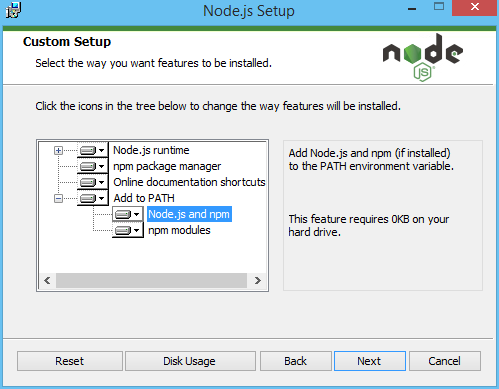
\includegraphics[scale=0.65]{images/node-installation}
	\caption{Configuración sugerida por el instalador de Node en Windows.}\label{fig:node-installation}
\end{figure}

Una vez terminada la instalación es posible ejecutar programas escritos en JavaScript en una computadora fuera del navegador.

\subsection{Ejemplos}

\subsubsection{Hello World}

\subsubsection{HTML Simple}

\section{Express}

\section{Bower}

\section{Boostrap}

\section{MongoDB}

MongoDB puede obtenerse desde el \href{https://www.mongodb.com/download-center}{centro de descargas} de su sitio web.\\

Su instalación en Windows es sencilla, sólo hay que ejecutar el paquete de instalación descargado y seguir la instalación recomendada. La instalación se realizará en el directorio \textit{C:/Program Files/MongoDB/Server/3.2} o similar, dependiendo de la versión instalada.\\

En la imagen \ref{fig:mongo-directory}, se observa el resultado de la instalación. Dentro de la carpeta \textit{bin} se encuentran los componentes principales y utilerías de MongoDB. Se recomienda la lectura del archivo README en el que se explica claramente la función de algunos de los componentes. 

\begin{figure}[H]
	\centering
	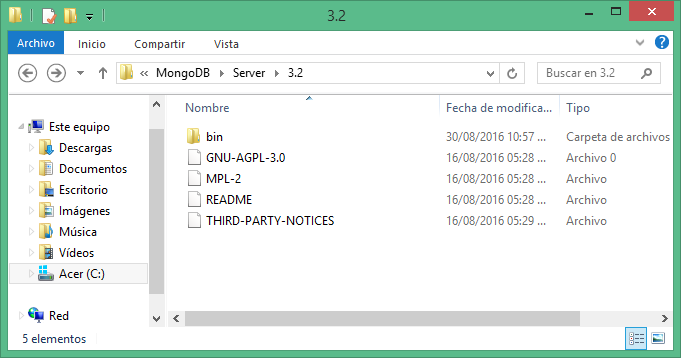
\includegraphics[scale=0.65]{images/mongo-installation-directory}
	\caption{Directorio de instalación de MongoDB}\label{fig:mongo-directory}
\end{figure}

Para poder hacer uso de Mongo desde el Command Prompt o Power Shell de Windows es necesario editar la variable de entorno PATH agregando la ruta de la carpeta \textit{bin} del directorio de instalación de Mongo.

Para modificar la variable PATH se pueden seguir \href{https://support.microsoft.com/en-us/kb/310519}{estos pasos}. En el paso 4 se selecciona la variable PATH, se da click en Editar y se agrega \textit{";C:/Program Files/MongoDB/Server/3.2/bin"} al final del valor de la variable.\\

Para poner a andar MongoDB se utiliza el ejecutable \textbf{mongod} acompañado de la opción \textbf{--dbpath  C:/../whatever/data/db}, esta opción indica al servicio de de Mongo cual es el directorio donde estarán o están contenidas las bases de datos. Es necesario que el directorio exista previo al inicio del servicio \textbf{mongod}.

En la figura \ref{fig:mongod-service} se observa el servicio de MongoDB en ejecución esperando por conexiones a través del puerto 27017, que es el puerto por defecto del servicio.\\

\begin{figure}[H]
	\centering
	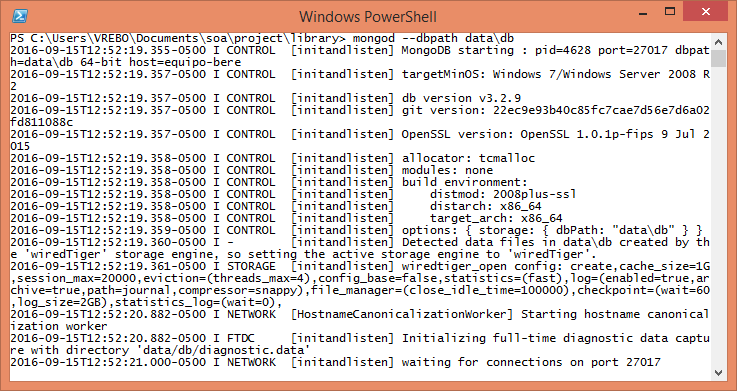
\includegraphics[scale=0.65]{images/mongo-service-started}
	\caption{Servicio mongod iniciado desde Windows Power Shell.}\label{fig:mongod-service}
\end{figure}

Ahora se puede ejecutar el cliente de MongoDB desde una línea de comandos para gestionar las colecciones de nuestras bases de datos.





\subsection{Mongoose}

\section{AngularJS}

\chapter{Desarrollo de una aplicación MEAN a través de servicios web REST}

\section{Descripción de la aplicación}
Para ejemplificar el uso del Stack MEAN y las herramientas antes descritas se desarrollará una aplicación web destinada a ser utilizada por bibliotecas. La aplicación permitirá por un lado, a la institución bibliotecaria hacer accesible el catálogo de su acervo a sus usuarios a través un sitio web, además los usuarios que hagan uso del servicio de préstamo de ejemplares a domicilio podrán consultar sus fechas de entrega por el mismo portal. 

\section{Estructura de la aplicación}
\section{Front-end}
\section{Esquema de la Base de Datos}
\section{API}
\section{Conexión Front-end Back-end}

\chapter{Seguridad}
\section{Seguridad a través de cuentas de usuario}
\section{Seguridad a través de Facebook}

\bibliographystyle{acm}
\bibliography{biblio}
\end{document}